\section{Segmentation of land zones}
\label{sec:segmentation}

Now that all fundamentals are covered, this chapter focuses on the implementation of the neural networks. Each reference architecture from section~\ref{sec:ref_archs} will be trained and evaluated with the original hyperparameters first. Afterwards, slight modifications are applied to the architectures, to look for optimization opportunities for the task at hand.

All implementation are done in Python with the popular Keras framework backed by TensorFlow~\cite{tf_whitepaper15}. It is a well established framework with extensive tooling, lots of documentation and a great open-source community. Also it is proven to be production-ready by a broad variety of companies for all kinds of tasks\footnote{Case studies can be found at \url{https://www.tensorflow.org/about/case-studies}}. More information about tools and hardware used throughout this thesis is listed in appendix~\ref{app:tools_hardware}

\subsection{Preparing the training and test dataset}
\label{sec:prepare_train_test}

Since the goal is to have a model that is able to generalize, it is recommended to measure its performance on data that it has not seen during training. Therefore, the dataset is split in two disjoint sets of data called \emph{training set} and \emph{test set}~\cite[p.~101f]{DLbook16}. During training, only samples from the training set are presented to the model. Afterwards, the performance is measured with samples from the test set. That way, models which just memorize the training examples perform rather bad compared to models which learn features on a generalized level.

The test set should only be used to evaluate the performance, but not decide on hyperparameters or architecture of the model. Otherwise, the model may become too closely aligned with the test set, i.~e. it is no longer possible to evaluate the generalization ability of the model with it. For such decisions another split of the training set is made, which is then called \emph{validation set}~\cite[p.~119]{DLbook16}. This set is used to estimate the generalization error during training and optimization without consulting the test set. Only after all optimizations have been done and no further changes to the model are planned, the test set is used to evaluate the final performance of the model.

There are many ways to pick the samples for the test and validation sets. \cite{val_split18} provides an insight into commonly used techniques. For this thesis, the test set respects the class imbalance that is found within the full dataset (see section~\ref{sec:dataset_considerations}). This is to achieve fair evaluation results which are not biased by any particular class. For each class, $10\%$ of the samples containing this class were chosen and added to the test set. The remaining samples are randomly distributed among training and validation set at a ratio of $9:1$.

\subsection{Tackling class imbalance}
\label{sec:class_imbalance}

As already expressed in section~\ref{sec:dataset_considerations}, there is a large imbalance between the segmentation classes in the dataset. This can lead to undesirable biases when training a model with such a dataset. For example, if the model predicts the \texttt{forest} class for every pixel all the time, the categorical accuracy would be at $65\%$ measured over the entire dataset. While this number does not sound too bad, the actual segmentation results would be useless.

There are some techniques to tackle the issues that come with an imbalanced dataset. One approach is to add class specific weights for the loss function during training~\cite{class_imbalance19}. The weights will affect the outcome of the loss function and therefore also the gradients during backpropagation. They are assigned antiproportionally to the distribution of the classes, i.~e. overrepresented classes are given small weights and underrepresented classes are given big weights. This has the same effect as duplicating the underrepresented samples in the training set, but it is computationally more efficient.

One major challenge is to find appropriate class weights, so that the imbalances are minimized as much as possible. For the given dataset, this can be done by taking into account the respective surface area for each class. Many different sets of class weights were tested, but none of them proved to be well suited. All trained models ended up predicting only a single class for all pixels all the time. Hence the class weights were dropped and not pursued any further.

At a closer look on the dataset, most segments are huge contiguous patches of the same class. The export of the image tiles as described in section~\ref{sec:image_export} results in a high number of images which only cover one single class. This might have a major impact on the learning outcome. Since most of the samples presented to the model only consist of a single class, it is very likely that the model aligns to this characteristics. So instead of learning to differentiate between segments with precise boundaries, the model might rather be directed to roughly classify larger areas.

For this reason, a different approach was chosen to address the class imbalance issues. Since the overall goal for the model is to differentiate between classes, images containing only a single class do not provide much value for training. Thus, all image tiles where all pixels belong to the same class are dropped entirely. One the one hand, this creates incentives for the model to better recognize the differences between classes and the characteristics of class boundaries. On the other hand, this also affects class imbalance, since large partitions of forests and agricultural areas are dropped, but mostly small streets and rivers are preserved. The first few attempts with the reduced training set looked    very promising. Hence, this strategy will be used further on for the training of all the models.

% TODO: add table with category distribution of multisegment and discuss it

\subsection{Experiments with U-Net}
\label{sec:unet_experiments}
The reference architecture that was explored first is the U-Net as introduced in section~\ref{sec:unet}. The architecture was implemented with the Keras framework. The code with all implementation details is listed in appendix~\ref{app:code}.

The default input size for images was set to $572\times 572$ pixels. Those are the same dimensions as the authors of U-Net used in their initial approach~\cite{unet15}. Because of the unpadded convolutional layers, the dimensions of the predictions are smaller than the original input image. For the standard configuration in U-Net the output size is $388\times 388$ pixels. Depending on the number of convolutional layers, these dimensions may vary.

All U-Net models were trained with a stochastic gradient descent optimizer. The initial learning rate was set to $0.1$ and reduced after every epoch, to allow finetuning of the weights towards the end of the training. A batch size of $4$ was used in combination with Nesterov momentum~\cite{nesterov83} of $0.99$ to speed up the training process and avoid oscillations. The loss was computed using a categorical crossentropy function.

Starting from the model with its original hyperparameter configuration, a few other configurations have been explored. To distinguish between the configurations, a naming convention is established. The original configuration is called \texttt{U-Net-23D}, where the number represents the exact number of convolutional layers in the model. The suffix \texttt{D} indicates that a dropout layer was added before the expansive path to provide regularization during the training.
% TODO: list configurations, give reasons for them

\subsubsection{Metrics}
During training, some metrics were collected to measure the predictive performance of the models (see section~\ref{sec:metrics} for details on the metrics). The plots in figure~\ref{fig:unet_train_metrics} present the epoch-wise loss, categorical accuracy and mean IoU for each U-Net configuration. The computation of the metrics was performed using the validation data set. This set only contains samples that were not fed into the model for updating its weights. Thus, the metrics provide good evidence for the model's ability to generalize.

\begin{figure}
    \newcommand{\UnetMetricsImageWidth}{0.32\textwidth}
    \centering
            \begin{scaletikzpicturetowidth}{\textwidth}
\begin{tikzpicture}[scale=\tikzscale]
    \begin{axis}[
        mark=x,
        cycle list name=mycolorlist,
        name=unetplot1,
        xmin=1, xmax=20,
    ]

    \addplot
    coordinates{
        (1, 1.3805760145187378)
        (2, 1.2029350996017456)
        (3, 1.0258171558380127)
        (4, 0.9140180349349976)
        (5, 0.8663129806518555)
        (6, 0.8311066627502441)
        (7, 0.8023157715797424)
        (8, 0.8315499424934387)
        (9, 0.7800722122192383)
        (10, 0.7648837566375732)
        (11, 0.7714964747428894)
        (12, 0.7677916884422302)
        (13, 0.7400503158569336)
        (14, 0.7427014708518982)
        (15, 0.7341839075088501)
        (16, 0.7475335001945496)
        (17, 0.7335283160209656)
        (18, 0.7399769425392151)
        (19, 0.7249587774276733)
        (20, 0.732405960559845)
    };

    \addplot
    coordinates{
        (1, 1.266666054725647)
        (2, 1.2810273170471191)
        (3, 1.1684550046920776)
        (4, 1.1036863327026367)
        (5, 0.9430841207504272)
        (6, 0.904362142086029)
        (7, 0.8709024786949158)
        (8, 0.8564851880073547)
        (9, 0.8495147228240967)
        (10, 0.8020780682563782)
        (11, 0.8123838305473328)
        (12, 0.8001933693885803)
        (13, 0.7681636810302734)
        (14, 0.7739695906639099)
        (15, 0.7636772394180298)
        (16, 0.7632151246070862)
        (17, 0.7528753876686096)
        (18, 0.746317982673645)
        (19, 0.7447842955589294)
        (20, 0.7457795143127441)
    };

    \addplot
    coordinates{
        (1, 1.2214372158050537)
        (2, 1.1931297779083252)
        (3, 1.1903798580169678)
        (4, 1.1395219564437866)
        (5, 1.1235227584838867)
        (6, 1.1210097074508667)
        (7, 1.1146382093429565)
        (8, 1.1130719184875488)
        (9, 1.1082816123962402)
        (10, 1.1061081886291504)
        (11, 1.1077511310577393)
        (12, 1.1041945219039917)
        (13, 1.1035878658294678)
        (14, 1.1043835878372192)
        (15, 1.1015698909759521)
        (16, 1.1020666360855103)
        (17, 1.1022522449493408)
        (18, 1.1018295288085938)
        (19, 1.1012828350067139)
        (20, 1.0986037254333496)
    };

    \addplot
    coordinates{
        (1, 1.3491429090499878)
        (2, 1.3386428356170654)
        (3, 1.3372877836227417)
        (4, 1.3367230892181396)
        (5, 1.3370440006256104)
    };

    \end{axis}
     \begin{axis}[
        mark=x,
        cycle list name=mycolorlist,
        name=unetplot2,
        at=(unetplot1.right of south east), anchor=left of south west,
        legend style={at={(0.5,-0.25)},anchor=north},
        xmin=1, xmax=20,
    ]

    \addplot
    coordinates{
        (1, 0.33829551935195923)
        (2, 0.501347541809082)
        (3, 0.645989179611206)
        (4, 0.685759425163269)
        (5, 0.7034950852394104)
        (6, 0.7160254120826721)
        (7, 0.7236952781677246)
        (8, 0.7100507020950317)
        (9, 0.728688657283783)
        (10, 0.7320661544799805)
        (11, 0.7301645874977112)
        (12, 0.7307804226875305)
        (13, 0.7398107051849365)
        (14, 0.7392005324363708)
        (15, 0.7434249520301819)
        (16, 0.7352943420410156)
        (17, 0.7410112023353577)
        (18, 0.742379903793335)
        (19, 0.7461361289024353)
        (20, 0.744171679019928)
    };
    \addlegendentry{U-Net-23D}

    \addplot
    coordinates{
        (1, 0.5139918327331543)
        (2, 0.4997938871383667)
        (3, 0.5388210415840149)
        (4, 0.5911301374435425)
        (5, 0.6690385341644287)
        (6, 0.6867047548294067)
        (7, 0.6966053247451782)
        (8, 0.7008607387542725)
        (9, 0.7030636668205261)
        (10 0.7222729325294495)
        (11, 0.7182477712631226)
        (12, 0.719925045967102)
        (13, 0.7313004732131958)
        (14, 0.7299023866653442)
        (15, 0.7342550754547119)
        (16, 0.7329625487327576)
        (17, 0.7349392175674438)
        (18, 0.7385514378547668)
        (19, 0.7386317253112793)
        (20, 0.7358725666999817)
    };
    \addlegendentry{U-Net-23}

    \addplot
    coordinates{
        (1, 0.5371174216270447)
        (2, 0.5497292876243591)
        (3, 0.5471416711807251)
        (4, 0.5873233675956726)
        (5, 0.6028231382369995)
        (6, 0.6036145091056824)
        (7, 0.6062009930610657)
        (8, 0.6073462963104248)
        (9, 0.6079839468002319)
        (10 0.6088585257530212)
        (11, 0.60825514793396)
        (12, 0.6091040968894958)
        (13, 0.609974205493927)
        (14, 0.6084813475608826)
        (15, 0.609819769859314)
        (16, 0.6098917722702026)
        (17, 0.6100775003433228)
        (18, 0.6097120046615601)
        (19, 0.6102020740509033)
        (20, 0.6107391715049744)
    };
    \addlegendentry{U-Net-18D}

    \addplot
    coordinates{
        (1, 0.35418376326560974)
        (2, 0.3636733293533325)
        (3, 0.35418376326560974)
        (4, 0.3549674451351166)
        (5, 0.3638293445110321)
    };
    \addlegendentry{U-Net-28D}

    % TODO: there are marks missing, check that
    \end{axis}

    \begin{axis}[
        mark=x,
        cycle list name=mycolorlist,
        at=(unetplot2.right of south east), anchor=left of south west,
        xmin=1, xmax=20,
    ]

    \addplot
    coordinates{
        (1, 0.05638260766863823)
        (2, 0.14802682399749756)
        (3, 0.26493558287620544)
        (4, 0.3173089921474457)
        (5, 0.34128832817077637)
        (6, 0.35409560799598694)
        (7, 0.3660319149494171)
        (8, 0.3550480306148529)
        (9, 0.3808368742465973)
        (10, 0.38574960827827454)
        (11, 0.38261398673057556)
        (12, 0.389729768037796)
        (13, 0.39931049942970276)
        (14, 0.3989291489124298)
        (15, 0.4041154682636261)
        (16, 0.40584757924079895)
        (17, 0.4110846519470215)
        (18, 0.4177403450012207)
        (19, 0.4257056713104248)
        (20, 0.4225998818874359)
    };

    \addplot
    coordinates{
        (1, 0.14475272595882416)
        (2, 0.13903780281543732)
        (3, 0.15666361153125763)
        (4, 0.2455795556306839)
        (5, 0.3087078332901001)
        (6, 0.3261967897415161)
        (7, 0.34233176708221436)
        (8, 0.3468801975250244)
        (9, 0.3550216257572174)
        (10, 0.37385615706443787)
        (11, 0.37024033069610596)
        (12, 0.3713560998439789)
        (13, 0.3893120288848877)
        (14, 0.3913959562778473)
        (15, 0.39039942622184753)
        (16, 0.4139955937862396)
        (17, 0.4096660614013672)
        (18, 0.41300487518310547)
        (19, 0.4125426113605499)
        (20, 0.42267632484436035)
    };

    \addplot
    coordinates{
        (1, 0.15161080658435822)
        (2, 0.1566145420074463)
        (3, 0.15519315004348755)
        (4, 0.1986483931541443)
        (5, 0.21347923576831818)
        (6, 0.2152184098958969)
        (7, 0.21574155986309052)
        (8, 0.21671517193317413)
        (9, 0.2158752679824829)
        (10, 0.21583761274814606)
        (11, 0.21597759425640106)
        (12, 0.21608270704746246)
        (13, 0.21780423820018768)
        (14, 0.21527351438999176)
        (15, 0.21591143310070038)
        (16, 0.21773125231266022)
        (17, 0.21799170970916748)
        (18, 0.21698665618896484)
        (19, 0.21827103197574615)
        (20, 0.21748535335063934)
    };

    \addplot
    coordinates{
        (1, 0.059030625969171524)
        (2, 0.06061220541596413)
        (3, 0.059030625969171524)
        (4, 0.059161242097616196)
        (5, 0.060638222843408585)
    };

    \end{axis}

    \node[align=center] at (3.3, -0.65) {\tiny loss};
    \node[align=center] at (11, -0.65) {\tiny cat. accuracy};
    \node[align=center] at (19, -0.65) {\tiny mean IoU};
\end{tikzpicture}
\end{scaletikzpicturetowidth}

    \caption{Training metrics of different variations of U-Net}
    \label{fig:unet_train_metrics}
\end{figure}

It is clearly visible that \texttt{U-Net-28D} does not perform well. For all three metrics it yields the worst results. Also, it does show any significant improvement over time, which is why the training was stopped after five epochs. On a closer investigation of the bad performance, it was found that the model always predicts the \texttt{agriculture} class for every pixel.
\WIP{Confidence for predictions? What is the root cause for this behavior? Too deep, so features are lost throughout the network?}
% TODO: calculate confidence, give reasons for this behavior
% buildings   0.21715826
% water   0.02491541
% forest   0.34937066
% traffic   0.01290903
% urban greens   0.03881836
% agriculture   0.35714394

The configuration \texttt{U-Net-18D} shows some improvements regarding the metrics in the first few epochs of training. After the fifth epoch the graphs flatten out and show only minor improvements. The training was stopped after ten epochs in total, where it hits around $60.8\%$ categorical accuracy and $21.6\%$ mean IoU. The \texttt{U-Net-18D} configuration was the one with the least number of parameters. Fewer parameters directly affect the ability to learn and generalize a broad range of features. The assumption is that the capacity of the model is not sufficient to comprehend the full space of features involved in this challenge.

The best results with regards to the metrics achieve both \texttt{U-Net-23D} and \texttt{U-Net-23}. They both show similar rates of improvements, which level out after $25$ epochs. The configuration with dropout layers features a slightly faster learning behavior, but both arrive at around $74\%$ categorical accuracy and $42.2\%$ mean IoU in the end.

The metrics already allow to draw some conclusions about the configurations. However, it is useful to also look at the visual results before starting the discussion.

\subsubsection{Images}
While the metrics provide a quick overview over larger parts of the data set, looking at concrete samples offers a deeper insight into the model's behavior in certain situations. Figure~\ref{fig:unet_prediction_images} depicts predictions in the test set from some configurations, together with the original image and the ground truth. The red square in the original image indicates the area that is covered in the prediction. As already raised in section~\ref{sec:dataset_considerations}, the ground truth labels are not super accurate with regards to the original image.

\begin{figure}
    \newcommand{\UnetPredictionsImageWidth}{0.18\textwidth}
    \centering

    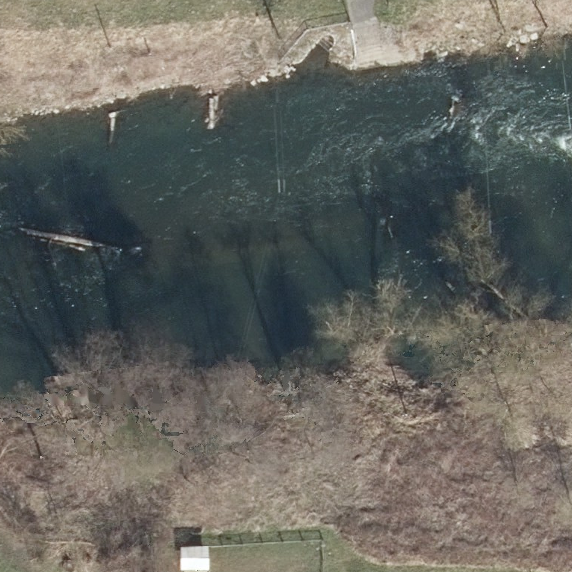
\includegraphics[width=\UnetPredictionsImageWidth]{images/unet/82607-image} \hfill
    
\includegraphics[width=\UnetPredictionsImageWidth]{images/unet/82607-label} \hfill
    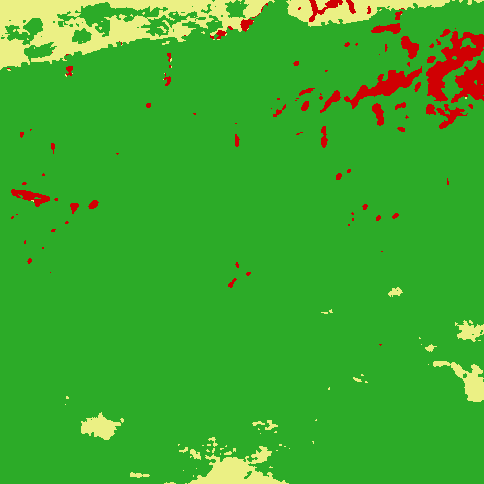
\includegraphics[width=\UnetPredictionsImageWidth]{images/unet/unet-18D/82607-prediction} \hfill
    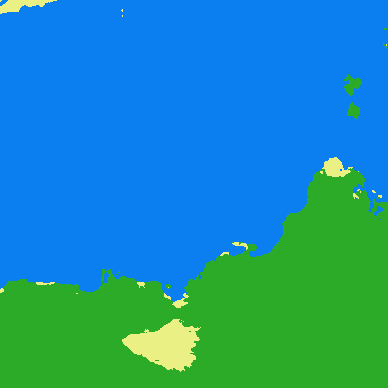
\includegraphics[width=\UnetPredictionsImageWidth]{images/unet/unet-23/82607-prediction} \hfill
    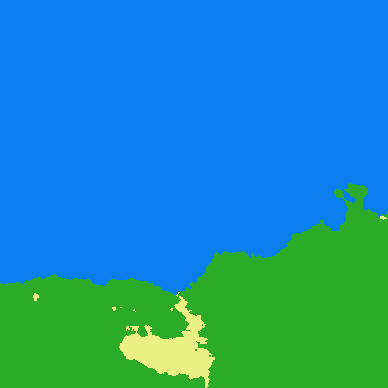
\includegraphics[width=\UnetPredictionsImageWidth]{images/unet/unet-23D/82607-prediction}

    \vspace{3mm}
    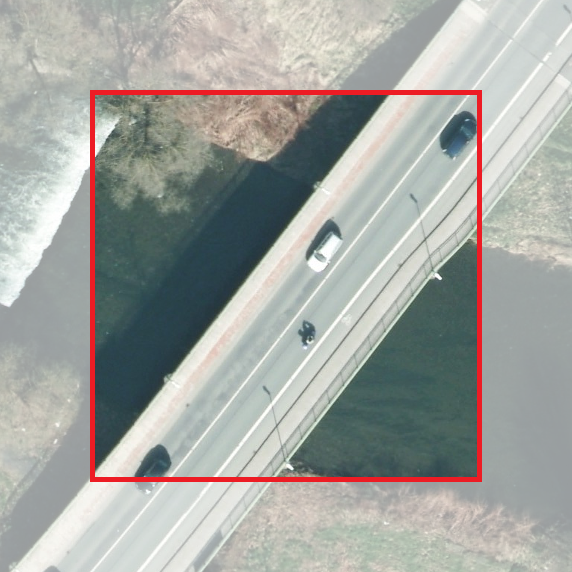
\includegraphics[width=\UnetPredictionsImageWidth]{images/unet/104483-image} \hfill
    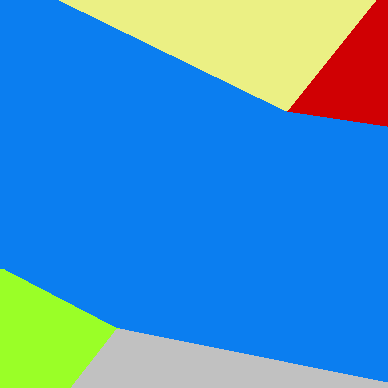
\includegraphics[width=\UnetPredictionsImageWidth]{images/unet/104483-label} \hfill
    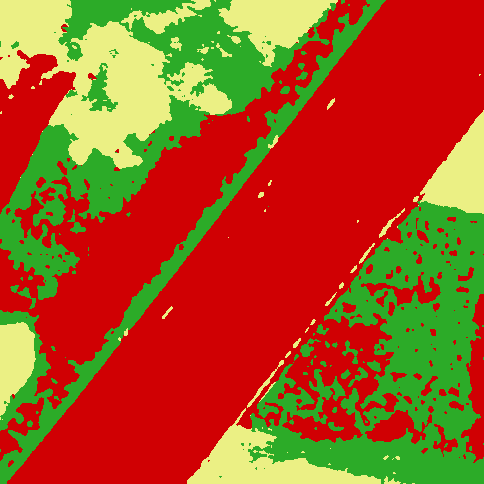
\includegraphics[width=\UnetPredictionsImageWidth]{images/unet/unet-18D/104483-prediction} \hfill
    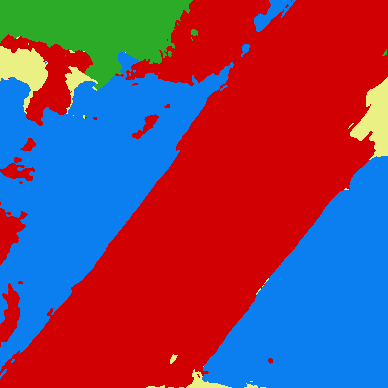
\includegraphics[width=\UnetPredictionsImageWidth]{images/unet/unet-23/104483-prediction} \hfill
    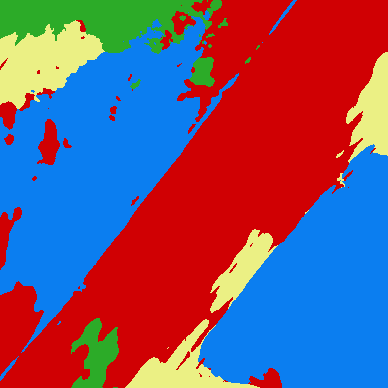
\includegraphics[width=\UnetPredictionsImageWidth]{images/unet/unet-23D/104483-prediction}

    \vspace{3mm}
    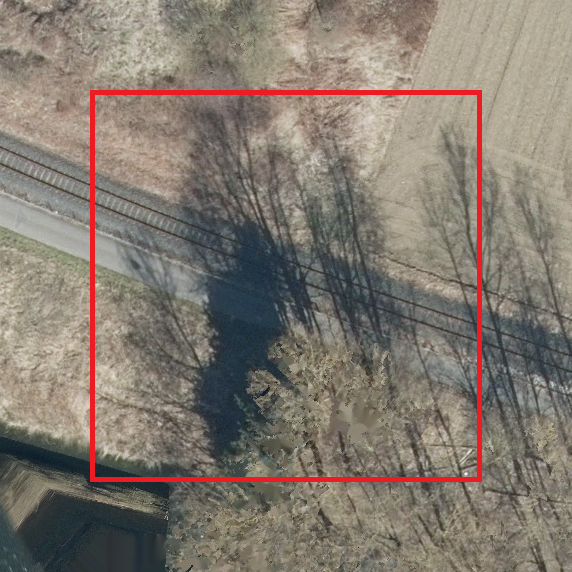
\includegraphics[width=\UnetPredictionsImageWidth]{images/unet/114975-image} \hfill
    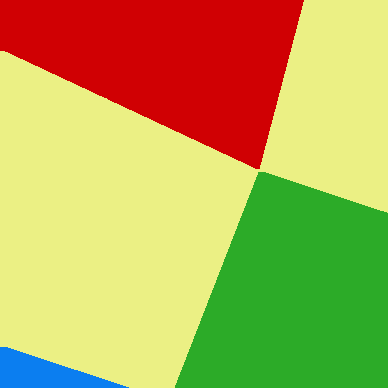
\includegraphics[width=\UnetPredictionsImageWidth]{images/unet/114975-label} \hfill
    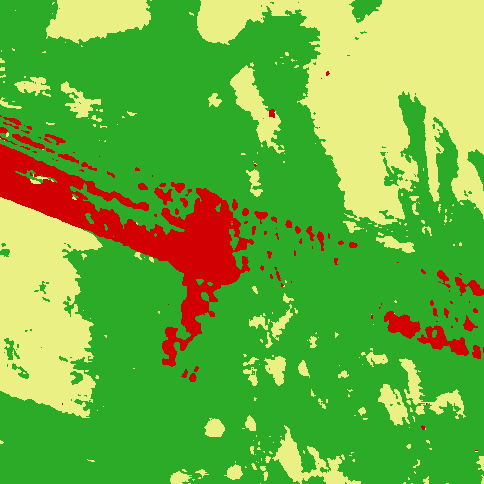
\includegraphics[width=\UnetPredictionsImageWidth]{images/unet/unet-18D/114975-prediction} \hfill
    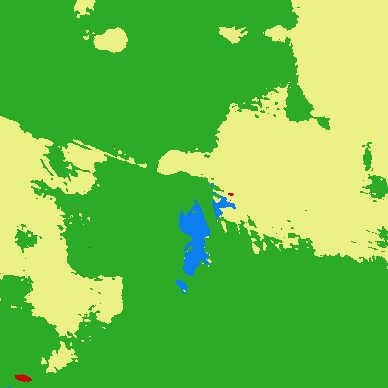
\includegraphics[width=\UnetPredictionsImageWidth]{images/unet/unet-23/114975-prediction} \hfill
    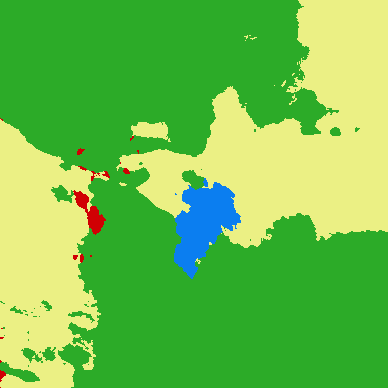
\includegraphics[width=\UnetPredictionsImageWidth]{images/unet/unet-23D/114975-prediction}

    \vspace{3mm}
    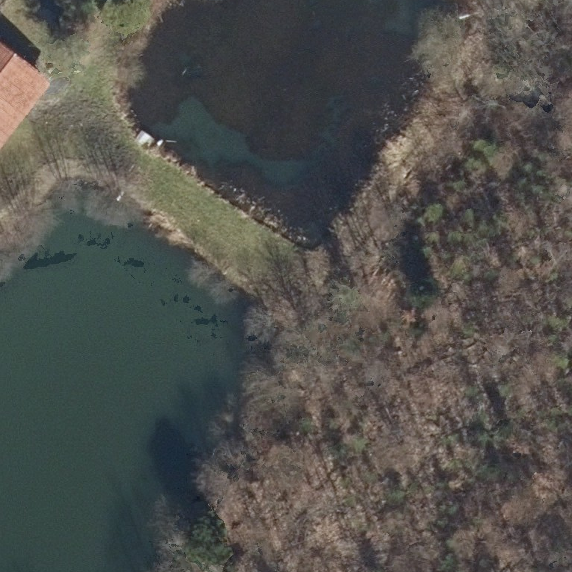
\includegraphics[width=\UnetPredictionsImageWidth]{images/unet/138625-image} \hfill
    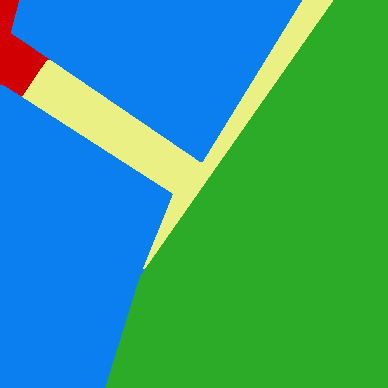
\includegraphics[width=\UnetPredictionsImageWidth]{images/unet/138625-label} \hfill
    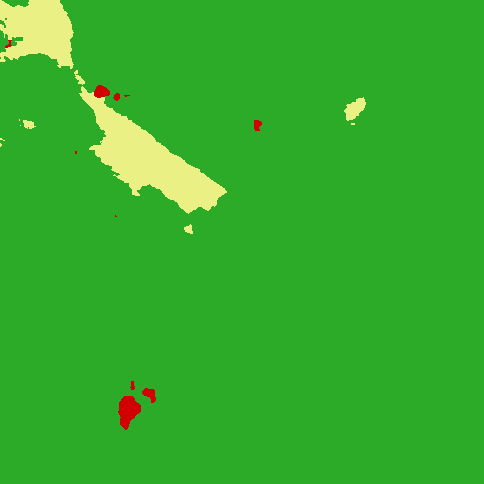
\includegraphics[width=\UnetPredictionsImageWidth]{images/unet/unet-18D/138625-prediction} \hfill
    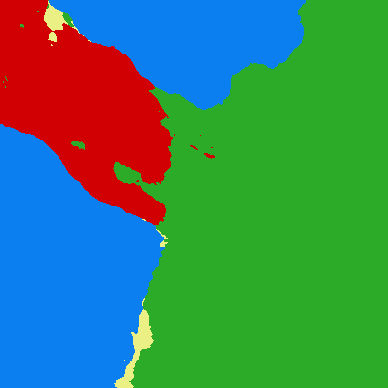
\includegraphics[width=\UnetPredictionsImageWidth]{images/unet/unet-23/138625-prediction} \hfill
    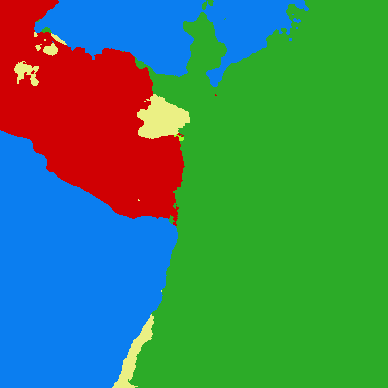
\includegraphics[width=\UnetPredictionsImageWidth]{images/unet/unet-23D/138625-prediction}

    \vspace{3mm}
    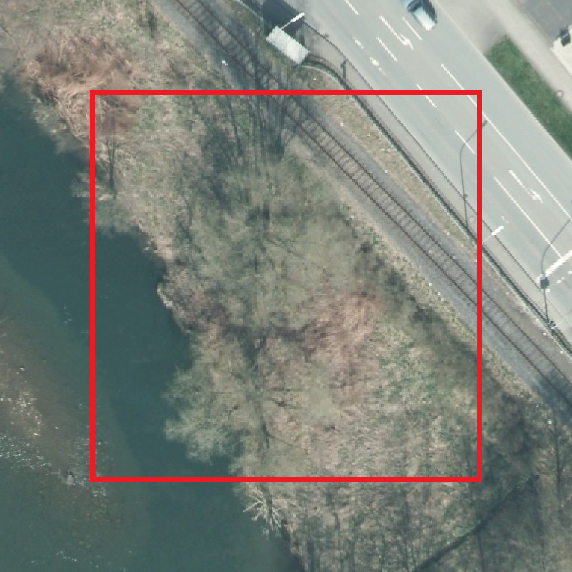
\includegraphics[width=\UnetPredictionsImageWidth]{images/unet/147352-image} \hfill
    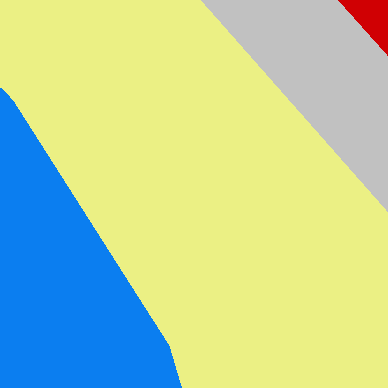
\includegraphics[width=\UnetPredictionsImageWidth]{images/unet/147352-label} \hfill
    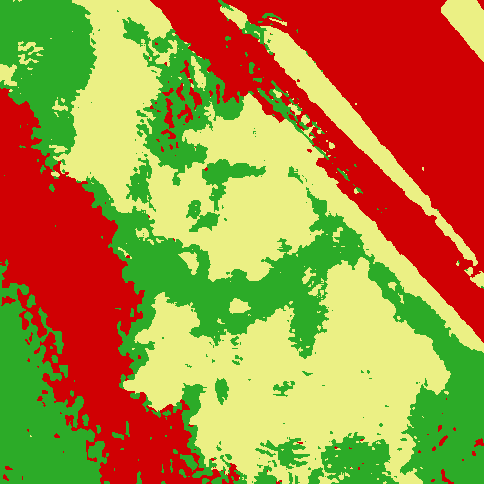
\includegraphics[width=\UnetPredictionsImageWidth]{images/unet/unet-18D/147352-prediction} \hfill
    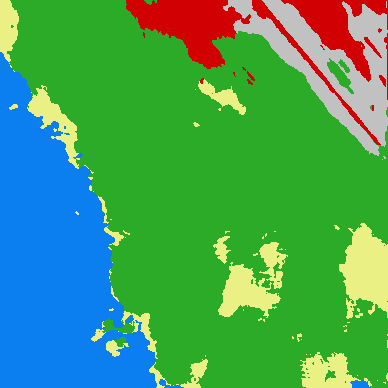
\includegraphics[width=\UnetPredictionsImageWidth]{images/unet/unet-23/147352-prediction} \hfill
    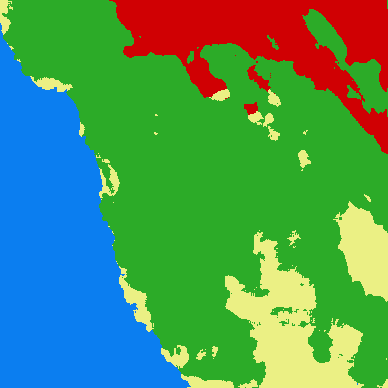
\includegraphics[width=\UnetPredictionsImageWidth]{images/unet/unet-23D/147352-prediction}

    \begin{tikzpicture}
        \node[align=center] at (-1.2, 0) {\tiny Input};
        \node[align=center] at (2.0, 0) {\tiny Ground Truth};
        \node[align=center] at (5.0, 0) {\tiny U-Net-18D};
        \node[align=center] at (8.1, 0) {\tiny U-Net-23};
        \node[align=center] at (11, 0) {\tiny U-Net-23D};
    \end{tikzpicture}
    \caption{Selected predictions of different configurations of U-Net}
    \label{fig:unet_prediction_images}
\end{figure}

The third column of the figure visualizes predictions of the \texttt{U-Net-18D} configuration. The predictions do not contain any \texttt{water} class. Instead, water bodies are predicted to be either \texttt{forest} or \texttt{buildings}. This explains why the categorical accuracy and mean IoU are lower compared to the \texttt{U-Net-23} configurations.

Both \texttt{U-Net-23} and \texttt{U-Net-23D} show better results for the \texttt{water} class. They are able to detect water surfaces correctly. However, sometimes shadows of other objects are also considered to be \texttt{water} (middle row). The first row shows that in some cases the predictions are even better than the labels.

All configurations struggle with the \texttt{traffic} class. In most situations, roads are incorrectly projected to \texttt{buildings}. Only \texttt{U-Net-23} has some correct predictions for the \texttt{traffic} class.

Based on the images shown in figure~\ref{fig:unet_prediction_images}, it is not possible to analyze the predictions with regards to the distinction between \texttt{forest} and \texttt{agriculture}. This will be considered later on in section~\ref{sec:segmentation_discussion}.

\subsection{Experiments with FC-DenseNet}
\label{sec:densenet_experiments}
In the next step, the FC-DenseNet reference architecture is investigated with regards to the segmentation challenge. Again, we analyze the original architecture like described in section~\ref{sec:densenet} as well as some variations with slightly modified hyperparameters.

For this architecture the dimensions of input and output are equally set to $224\times 224$. Since the convolutional layers in this architecture use padding, the dimensions are independent from the number of layers.

The loss is again calculated by a categorical crossentropy function. During training, the weight updates are applied using a RMSprop~\cite{rmsprop14} optimizer. The learning rate is initialized with $0.001$ (according to~\cite{denseseg17}) and decreased after each epoch.

Another naming convention is applied to distinguish the variations of the FC-DenseNet models. The reference model is called \texttt{FCDN-103D}, again indicating the number of convolutional layers and the use of dropout. The letter \texttt{C} denotes the application of compression layers before transition-down layers to condense the outputs of dense blocks (see~\cite{denseseg17} for details). The compression rate of those layers is set to $0.5$, i.~e. the number of feature maps is halved.
% TODO: list configurations, give reasons for them

\subsubsection{Metrics}
The training metrics for all FC-DenseNet configurations are presented in figure~\ref{fig:densenet_train_metrics}. Although there are some strong oscillations, most of the configurations show ongoing improvements over the course of 20 epochs. Towards the end of the training the oscillations faint and the graphs converge.

\begin{figure}
    \newcommand{\DensenetMetricsImageWidth}{0.32\textwidth}
    \centering
            \begin{scaletikzpicturetowidth}{\textwidth}
\begin{tikzpicture}[scale=\tikzscale]
    \begin{axis}[
        mark=x,
        cycle list name=mycolorlist,
        name=densenetplot1,
        xmin=1, xmax=20,
    ]

    \addplot
    coordinates{
        (1, 1.8778098821640015)
        (2, 1.2668427228927612)
        (3, 1.2766574621200562)
        (4, 1.4314723014831543)
        (5, 1.4286470413208008)
        (6, 1.3057966232299805)
        (7, 1.2254855632781982)
        (8, 1.4993059635162354)
        (9, 1.1675904989242554)
        (10, 1.490395188331604)
        (11, 1.2040382623672485)
        (12, 1.4405009746551514)
        (13, 1.3286089897155762)
        (14, 1.210574984550476)
        (15, 1.1925950050354004)
        (16, 1.3692342042922974)
        (17, 1.2186700105667114)
        (18, 1.2532116174697876)
        (19, 1.1861357688903809)
        (20, 1.168188214302063)
    };

    \addplot
    coordinates{
        (1, 2.1999971866607666)
        (2, 1.3902311325073242)
        (3, 1.3412078619003296)
        (4, 1.2981048822402954)
        (5, 1.280882716178894)
        (6, 1.2695380449295044)
        (7, 1.3394079208374023)
        (8, 1.2355924844741821)
        (9, 1.2429777383804321)
        (10, 1.3308765888214111)
        (11, 1.2678800821304321)
        (12, 1.2725298404693604)
        (13, 1.3483526706695557)
        (14, 1.3196649551391602)
        (15, 1.2746803760528564)
        (16, 1.3376092910766602)
        (17, 1.3442707061767578)
        (18, 1.327423095703125)
        (19, 1.2989463806152344)
        (20, 1.2952357530593872)
    };

    \addplot
    coordinates{
        (1, 2.3974061012268066)
        (2, 1.3469152450561523)
        (3, 1.3552826642990112)
        (4, 1.326025128364563)
        (5, 1.3972184658050537)
        (6, 1.316970944404602)
        (7, 1.295585036277771)
        (8, 1.3838255405426025)
        (9, 1.2869324684143066)
        (10, 1.3071309328079224)
        (11, 1.3551321029663086)
        (12, 1.3308088779449463)
        (13, 1.375392198562622)
        (14, 1.34626042842865)
        (15, 1.3224772214889526)
        (16, 1.3284034729003906)
        (17, 1.3779839277267456)
        (18, 1.3398308753967285)
        (19, 1.3465551137924194)
        (20, 1.3300797939300537)
    };

    \addplot
    coordinates{
        (1, 1.990792155265808)
        (2, 1.294736623764038)
        (3, 1.2612152099609375)
        (4, 1.2450172901153564)
        (5, 1.24184250831604)
        (6, 1.2792901992797852)
        (7, 1.2662909030914307)
        (8, 1.37437903881073)
        (9, 1.2648396492004395)
        (10, 1.2657694816589355)
        (11, 1.316687822341919)
        (12, 1.4254909753799438)
        (13, 1.2919646501541138)
        (14, 1.3055157661437988)
        (15, 1.285273790359497)
        (16, 1.3169896602630615)
        (17, 1.3447442054748535)
        (18, 1.303223967552185)
        (19, 1.2977485656738281)
        (20, 1.2806230783462524)
    };

    \end{axis}
     \begin{axis}[
        mark=x,
        cycle list name=mycolorlist,
        name=densenetplot2,
        at=(densenetplot1.right of south east), anchor=left of south west,
        legend style={at={(0.5,-0.25)},anchor=north},
        xmin=1, xmax=20,
    ]

    \addplot
    coordinates{
        (1, 0.44403234124183655)
        (2, 0.5382390022277832)
        (3, 0.5460906624794006)
        (4, 0.5117834806442261)
        (5, 0.49210643768310547)
        (6, 0.5355142951011658)
        (7, 0.5704494714736938)
        (8, 0.4416641891002655)
        (9, 0.6110737323760986)
        (10, 0.4632301926612854)
        (11, 0.590806782245636)
        (12, 0.5226526260375977)
        (13, 0.5564858317375183)
        (14, 0.5993890166282654)
        (15, 0.613778829574585)
        (16, 0.5397917628288269)
        (17, 0.5880735516548157)
        (18, 0.5896559357643127)
        (19, 0.6149882078170776)
        (20, 0.6262763142585754)
    };
    \addlegendentry{FC-DenseNet-103D}

    \addplot
    coordinates{
        (1, 0.31083741784095764)
        (2, 0.4629298746585846)
        (3, 0.47024381160736084)
        (4, 0.5197407603263855)
        (5, 0.5138208270072937)
        (6, 0.5358591675758362)
        (7, 0.4863249957561493)
        (8, 0.5566446781158447)
        (9, 0.5620558261871338)
        (10, 0.49684542417526245)
        (11, 0.5612539649009705)
        (12, 0.5544501543045044)
        (13, 0.5163871049880981)
        (14, 0.5430474281311035)
        (15, 0.5622951984405518)
        (16, 0.5312788486480713)
        (17, 0.5277349352836609)
        (18, 0.5413538217544556)
        (19, 0.5542507767677307)
        (20, 0.5590786933898926)
    };
    \addlegendentry{FC-DenseNet-103CD}

    \addplot
    coordinates{
        (1, 0.24311639368534088)
        (2, 0.4761204421520233)
        (3, 0.4544506072998047)
        (4, 0.4913800060749054)
        (5, 0.41295066475868225)
        (6, 0.5058783292770386)
        (7, 0.5192673206329346)
        (8, 0.4526740610599518)
        (9, 0.5332894325256348)
        (10, 0.5307732820510864)
        (11, 0.5094674229621887)
        (12, 0.5299655795097351)
        (13, 0.49733099341392517)
        (14, 0.5140370726585388)
        (15, 0.5340467691421509)
        (16, 0.525802493095398)
        (17, 0.499888151884079)
        (18, 0.5290431976318359)
        (19, 0.5265495777130127)
        (20, 0.5373263955116272)
    };
    \addlegendentry{FC-DenseNet-67D}

    \addplot
    coordinates{
        (1, 0.3250448405742645)
        (2, 0.5240246057510376)
        (3, 0.5330521464347839)
        (4, 0.5476676821708679)
        (5, 0.5379430651664734)
        (6, 0.5243373513221741)
        (7, 0.5286471247673035)
        (8, 0.47282737493515015)
        (9, 0.5424470901489258)
        (10, 0.5523974299430847)
        (11, 0.5108893513679504)
        (12, 0.5004795789718628)
        (13, 0.5263856053352356)
        (14, 0.5332449078559875)
        (15, 0.5562388896942139)
        (16, 0.534349262714386)
        (17, 0.5274752974510193)
        (18, 0.5481530427932739)
        (19, 0.5545112490653992)
        (20, 0.5611099600791931)
    };
    \addlegendentry{FC-DenseNet-56D}

    \end{axis}

    \begin{axis}[
        mark=x,
        cycle list name=mycolorlist,
        at=(densenetplot2.right of south east), anchor=left of south west,
        xmin=1, xmax=20,
        ymin=0, ymax=0.35,
    ]

    \addplot
    coordinates{
        (1, 0.15961624681949615)
        (2, 0.23034006357192993)
        (3, 0.2510993778705597)
        (4, 0.2040325254201889)
        (5, 0.15874336659908295)
        (6, 0.2393379658460617)
        (7, 0.2576610743999481)
        (8, 0.20172123610973358)
        (9, 0.28852298855781555)
        (10, 0.1903650313615799)
        (11, 0.2816150486469269)
        (12, 0.2380661964416504)
        (13, 0.2526349425315857)
        (14, 0.28796717524528503)
        (15, 0.29596516489982605)
        (16, 0.2512836754322052)
        (17, 0.2903881371021271)
        (18, 0.28366556763648987)
        (19, 0.30205875635147095)
        (20, 0.28375494480133057)
    };

    \addplot
    coordinates{
        (1, 0.08612015843391418)
        (2, 0.18902510404586792)
        (3, 0.18584029376506805)
        (4, 0.2238929122686386)
        (5, 0.21692800521850586)
        (6, 0.2446306347846985)
        (7, 0.19728021323680878)
        (8, 0.254301518201828)
        (9, 0.2588264048099518)
        (10, 0.21687805652618408)
        (11, 0.2554681599140167)
        (12, 0.24556516110897064)
        (13, 0.21257217228412628)
        (14, 0.23620039224624634)
        (15, 0.23790551722049713)
        (16, 0.2152477353811264)
        (17, 0.2248375415802002)
        (18, 0.2260301262140274)
        (19, 0.2301390916109085)
        (20, 0.240129753947258)
    };

    \addplot
    coordinates{
        (1, 0.05528780445456505)
        (2, 0.2058449238538742)
        (3, 0.1926068663597107)
        (4, 0.1960599273443222)
        (5, 0.1480538696050644)
        (6, 0.21407771110534668)
        (7, 0.22343073785305023)
        (8, 0.1498967856168747)
        (9, 0.21587294340133667)
        (10, 0.23544591665267944)
        (11, 0.21624718606472015)
        (12, 0.21524637937545776)
        (13, 0.1991012543439865)
        (14, 0.2097732275724411)
        (15, 0.2226145714521408)
        (16, 0.21674305200576782)
        (17, 0.21302568912506104)
        (18, 0.21026158332824707)
        (19, 0.22532594203948975)
        (20, 0.23161913454532623)
    };

    \addplot
    coordinates{
        (1, 0.13292203843593597)
        (2, 0.22567109763622284)
        (3, 0.23399783670902252)
        (4, 0.2489478588104248)
        (5, 0.19032984972000122)
        (6, 0.2309076339006424)
        (7, 0.2147936075925827)
        (8, 0.1856151819229126)
        (9, 0.20955342054367065)
        (10, 0.24931295216083527)
        (11, 0.20019109547138214)
        (12, 0.17687444388866425)
        (13, 0.18552462756633759)
        (14, 0.19671611487865448)
        (15, 0.21579863131046295)
        (16, 0.1941973716020584)
        (17, 0.21591031551361084)
        (18, 0.20780526101589203)
        (19, 0.2145579308271408)
        (20, 0.21770614385604858)
    };

    \end{axis}

    \node[align=center] at (3.3, -0.65) {\tiny loss};
    \node[align=center] at (11, -0.65) {\tiny cat. accuracy};
    \node[align=center] at (19, -0.65) {\tiny mean IoU};
\end{tikzpicture}
\end{scaletikzpicturetowidth}

    \caption{Training metrics of different variations of FC-DenseNet}
    \label{fig:densenet_train_metrics}
\end{figure}

This behavior is a sign that the initial learning rate was set too high. The weights in the model are then adjusted too drastically, so that minima of the loss function are skipped. The learning rate shrinks towards the end of the training, which explains the reduced oscillations.

According to figure~\ref{fig:densenet_train_metrics}, \texttt{FCDN-103D} yields the best results. At the end of the training the metrics are at a loss of $1.17$, categorical accuracy of $62.6\%$ and mean IoU of $28.4\%$. Those numbers are substantially better than the other configurations, which probably relies on the fact that this configuration also has the highest number of parameters.

The other three configurations report fairly uniform results in terms of metrics. This is very interesting with regards to performance and computational efficiency. \texttt{FCDN-103DC} has more than twice the number of parameters than \texttt{FCDN-56D} ($5.9~\text{M}$ compared to $2.7~\text{M}$) and still many more than \texttt{FCDN-67D} ($4.0~\text{M}$). This means that the configurations with fewer parameters store their information much more efficiently.

\subsubsection{Images}
Figure~\ref{fig:densenet_prediction_images} shows some sample predictions made by the FC-DenseNet configuration. The original images and ground truth labels are included for reference. All images were taken from the test data set.

\begin{figure}
    \newcommand{\DensenetPredictionsImageWidth}{0.15\textwidth}
    \centering

    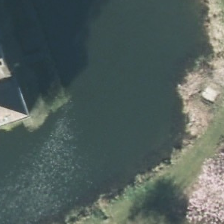
\includegraphics[width=\DensenetPredictionsImageWidth]{images/densenet/101444-image} \hfill
    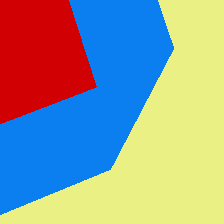
\includegraphics[width=\DensenetPredictionsImageWidth]{images/densenet/101444-label} \hfill
    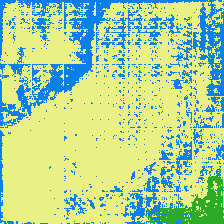
\includegraphics[width=\DensenetPredictionsImageWidth]{images/densenet/densenet-103D/101444-prediction} \hfill
    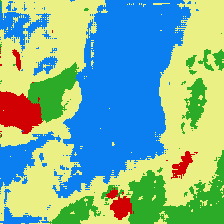
\includegraphics[width=\DensenetPredictionsImageWidth]{images/densenet/densenet-103CD/101444-prediction} \hfill
    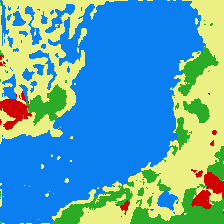
\includegraphics[width=\DensenetPredictionsImageWidth]{images/densenet/densenet-67D/101444-prediction} \hfill
    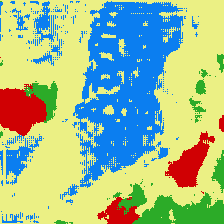
\includegraphics[width=\DensenetPredictionsImageWidth]{images/densenet/densenet-56D/101444-prediction}

    \vspace{3mm}
    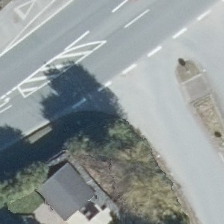
\includegraphics[width=\DensenetPredictionsImageWidth]{images/densenet/291991-image} \hfill
    
\includegraphics[width=\DensenetPredictionsImageWidth]{images/densenet/291991-label} \hfill
    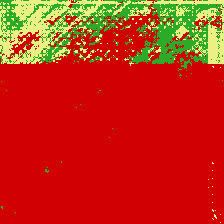
\includegraphics[width=\DensenetPredictionsImageWidth]{images/densenet/densenet-103D/291991-prediction} \hfill
    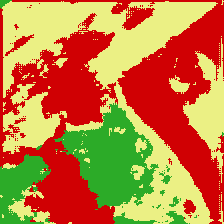
\includegraphics[width=\DensenetPredictionsImageWidth]{images/densenet/densenet-103CD/291991-prediction} \hfill
    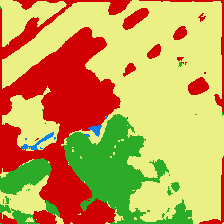
\includegraphics[width=\DensenetPredictionsImageWidth]{images/densenet/densenet-67D/291991-prediction} \hfill
    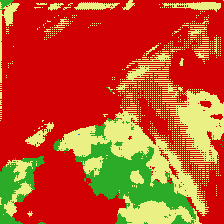
\includegraphics[width=\DensenetPredictionsImageWidth]{images/densenet/densenet-56D/291991-prediction}

    \vspace{3mm}
    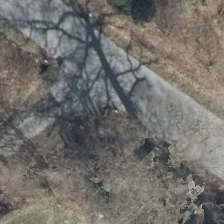
\includegraphics[width=\DensenetPredictionsImageWidth]{images/densenet/436897-image} \hfill
    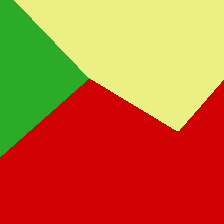
\includegraphics[width=\DensenetPredictionsImageWidth]{images/densenet/436897-label} \hfill
    
\includegraphics[width=\DensenetPredictionsImageWidth]{images/densenet/densenet-103D/436897-prediction} \hfill
    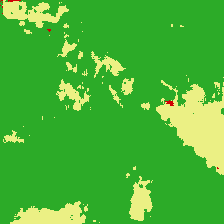
\includegraphics[width=\DensenetPredictionsImageWidth]{images/densenet/densenet-103CD/436897-prediction} \hfill
    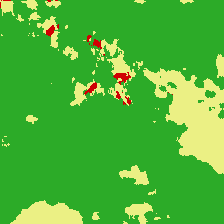
\includegraphics[width=\DensenetPredictionsImageWidth]{images/densenet/densenet-67D/436897-prediction} \hfill
    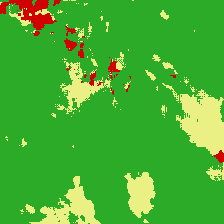
\includegraphics[width=\DensenetPredictionsImageWidth]{images/densenet/densenet-56D/436897-prediction}

    \vspace{3mm}
    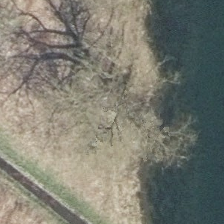
\includegraphics[width=\DensenetPredictionsImageWidth]{images/densenet/626312-image} \hfill
    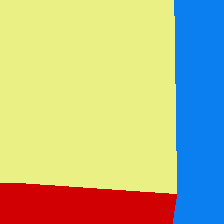
\includegraphics[width=\DensenetPredictionsImageWidth]{images/densenet/626312-label} \hfill
    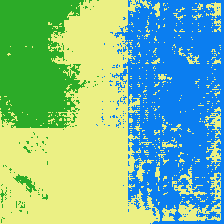
\includegraphics[width=\DensenetPredictionsImageWidth]{images/densenet/densenet-103D/626312-prediction} \hfill
    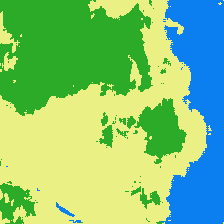
\includegraphics[width=\DensenetPredictionsImageWidth]{images/densenet/densenet-103CD/626312-prediction} \hfill
    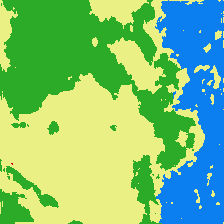
\includegraphics[width=\DensenetPredictionsImageWidth]{images/densenet/densenet-67D/626312-prediction} \hfill
    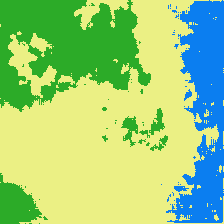
\includegraphics[width=\DensenetPredictionsImageWidth]{images/densenet/densenet-56D/626312-prediction}

    \vspace{3mm}
    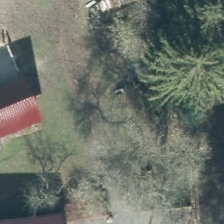
\includegraphics[width=\DensenetPredictionsImageWidth]{images/densenet/768909-image} \hfill
    \includegraphics[width=\DensenetPredictionsImageWidth]{images/densenet/768909-label} \hfill
    \includegraphics[width=\DensenetPredictionsImageWidth]{images/densenet/densenet-103D/768909-prediction} \hfill
    \includegraphics[width=\DensenetPredictionsImageWidth]{images/densenet/densenet-103CD/768909-prediction} \hfill
    \includegraphics[width=\DensenetPredictionsImageWidth]{images/densenet/densenet-67D/768909-prediction} \hfill
    \includegraphics[width=\DensenetPredictionsImageWidth]{images/densenet/densenet-56D/768909-prediction}

    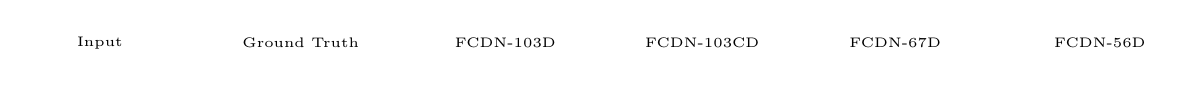
\begin{tikzpicture}
        \node[align=center] at (0, 0) {};
        \node[align=center] at (0.8, 0) {\tiny Input};
        \node[align=center] at (3.35, 0) {\tiny Ground Truth};
        \node[align=center] at (5.95, 0) {\tiny FCDN-103D};
        \node[align=center] at (8.45, 0) {\tiny FCDN-103CD};
        \node[align=center] at (10.9, 0) {\tiny FCDN-67D};
        \node[align=center] at (13.5, 0) {\tiny FCDN-56D};
    \end{tikzpicture}
    \caption{Selected predictions of different configurations of FC-DenseNet}
    \label{fig:densenet_prediction_images}
\end{figure}

While \texttt{FCDN-103D} performed very well in the metrics, the actual results have some shortcomings. The segments are not separated clearly and form some very fragmented regions. In order to use these predictions meaningfully, they would first have to be smoothed out. The same observations apply in an attenuated form to \texttt{FCDN-56D}. The  other two configurations do not exhibit this behavior.

None of the configurations was able to predict the \texttt{traffic} class correctly. Mostly it is confused with the \texttt{buildings} class.

From a purely visual point of view \texttt{FCDN-103CD} and \texttt{FCDN-67D} deliver the best results. Especially the predictions for the \texttt{water} class seem very promising.

The differentiation between the \texttt{agriculture} and \texttt{forest} classes is noticeable. In reality, the transition between those two classes is seamless and hardly perceivable. So it is expected that the predictions are subject to minor fluctuations.

\subsection{Experiments with W-Net}
\label{sec:wnet_experiments}
Lastly, the W-Net architecture presented in section~\ref{sec:wnet} is implemented. For that, big parts of the U-Net implementation could be reused, because W-Net essentially consists of two subsequent U-Nets. In contrast to the original U-Net architecture however, the W-Net employs zero padding for the convolutional layers, so that input and output dimensions are equal.

The W-Net architecture was designed for unsupervised training. This means, the labels of the data set are not consulted during training. Instead, the original images are used as both input and label. This way, the model has to learn an appropriate distribution of classes all by itself. Since this setup allows for arbitrary numbers of classes, the number is appended to the model name as a suffix. Otherwise, the naming convention is the same as for U-Net in section~\ref{sec:unet_experiments}.

Unlike the original architecture proposed in~\cite{wnet17} the training function was not split in two parts. Instead, the output of the encoder was altered to represent a clean one-hot encoding of the class with the highest prediction. This was done for two reasons:

First, that way the decoder only has $n$ distinct values from which it has to reconstruct the image (where $n$ is the number of classes). Thus, it is not possible to use intermediate vectors to encode additional states. This makes image reconstruction for the decoder a lot harder.

Additionally, the classes predicted by the encoder have to be picked very carefully in order to allow any meaningful reconstruction of the images at all. The goal is that the encoder is really sophisticated with regards to class predictions.

As a part of the thesis, many different options were explored for the optimizer and loss function to use for training. In the end, the results were all equally weak. The configurations presented in the next sections were trained using an Adam optimizer with a learning rate of $0.001$ and a categorical crossentropy loss function.

\subsubsection{Metrics}
The metrics for W-Net are different from the ones presented for U-Net and FC-DenseNet. Since no labels were used during training, it is not possible to calculate the categorical accuracy and mean IoU. This is because the class predictions learned by the encoder do not necessarily match with the predefined classes in the labels.

\begin{figure}
    \centering
            \begin{scaletikzpicturetowidth}{\textwidth}
\begin{tikzpicture}[scale=0.65]
     \begin{axis}[
        mark=x,
        cycle list name=mycolorlist,
        legend style={at={(0.5,-0.25)},anchor=north},
        xmin=0, xmax=5000,
    ]

    \addplot
    coordinates{
        (0, 1.530838597)
        (250, 1.496959729)
        (500, 1.506180048)
        (750, 1.509707813)
        (1000, 1.510138181)
        (1250, 1.513259780)
        (1500, 1.514958584)
        (1750, 1.513588905)
        (2000, 1.514086481)
        (2250, 1.512764335)
        (2500, 1.516359918)
        (2750, 1.514419317)
        (3000, 1.515940614)
        (3250, 1.512393255)
        (3500, 1.513636075)
        (3750, 1.512662097)
        (4000, 1.512252454)
        (4250, 1.513413423)
        (4500, 1.514070868)
        (4750, 1.514217734)
    };
    \addlegendentry{W-Net-36D-6}

    \addplot
    coordinates{
        (0, 1.526545445)
        (250, 1.498251622)
        (500, 1.507898344)
        (750, 1.509821892)
        (1000, 1.512769361)
        (1250, 1.512696606)
        (1500, 1.513341665)
        (1750, 1.515551324)
        (2000, 1.510578221)
        (2250, 1.512840509)
        (2500, 1.515694106)
        (2750, 1.514492752)
        (3000, 1.514587283)
        (3250, 1.514625147)
        (3500, 1.512107372)
        (3750, 1.510750664)
        (4000, 1.512461345)
        (4250, 1.513934228)
        (4500, 1.514142394)
        (4750, 1.515447481)
    };
    \addlegendentry{W-Net-46D-6}

    \addplot
    coordinates{
        (0, 1.525186402)
        (250, 1.497649679)
        (500, 1.504152746)
        (750, 1.508339763)
        (1000, 1.509541966)
        (1250, 1.512159856)
        (1500, 1.511834502)
        (1750, 1.511816302)
        (2000, 1.509140187)
        (2250, 1.510403678)
        (2500, 1.513000253)
        (2750, 1.512940407)
        (3000, 1.511894814)
        (3250, 1.511292121)
        (3500, 1.512401742)
        (3750, 1.512220313)
        (4000, 1.511644959)
        (4250, 1.512246013)
        (4500, 1.512521386)
        (4750, 1.513722123)
    };
    \addlegendentry{W-Net-36D-20}

    \addplot
    coordinates{
        (0, 1.535486313)
        (250, 1.500401722)
        (500, 1.506174445)
        (750, 1.509697914)
        (1000, 1.512826447)
        (1250, 1.513225843)
        (1500, 1.512589696)
        (1750, 1.512383233)
        (2000, 1.512146653)
        (2250, 1.513534832)
        (2500, 1.514685636)
        (2750, 1.516164322)
        (3000, 1.514503598)
        (3250, 1.512789011)
        (3500, 1.512024403)
        (3750, 1.510563542)
        (4000, 1.511181457)
        (4250, 1.511881276)
        (4500, 1.514057517)
        (4750, 1.514203548)
    };
    \addlegendentry{W-Net-46D-20}

    \end{axis}

    \node[align=center] at (3.3, -0.65) {\tiny loss};
\end{tikzpicture}
\end{scaletikzpicturetowidth}

    \caption{Training metrics of different variations of W-Net}
    \label{fig:wnet_train_metrics}
\end{figure}

The only metric shown in figure~\ref{fig:wnet_train_metrics} is the categorical crossentropy loss during training. Since no configuration has major improvements (note the small range on the y-axis), training is stopped after a single epoch. Thus, the graph plots the loss per batch in the training set.

All configurations show similar behavior during the training. Over the first few batches of data, there is an adequate improvement on the loss. Only after a few more batches, the predictions become worse again. Interestingly, the graphs for all configurations look like they all follow the same pattern. At the time of writing, no safisfying explanation can be given for those incidents.

\subsubsection{Images}
Figure~\ref{fig:wnet_prediction_images} lists some visual results of the W-Net configurations extracted from the test set. For each configuration two images are displayed. The first one is the predicted class segmentation. The class colors in the predictions are not related to any of the classes mentioned earlier. They rather represent what the respective encoder learned to differentiate in the images. The second image is the reconstruction of the original image predicted by the decoder from the class segmentation.

\begin{figure}
    \newcommand{\WnetPredictionsImageWidth}{0.10\textwidth}
    \centering

    \includegraphics[width=\WnetPredictionsImageWidth]{images/wnet/original/19743-image} \hfill
    \includegraphics[width=\WnetPredictionsImageWidth]{images/wnet/36d-6/19743-prediction} \hfill
    \includegraphics[width=\WnetPredictionsImageWidth]{images/wnet/36d-6/19743-restored} \hfill
    \includegraphics[width=\WnetPredictionsImageWidth]{images/wnet/46d-6/19743-prediction} \hfill
    \includegraphics[width=\WnetPredictionsImageWidth]{images/wnet/46d-6/19743-restored} \hfill
    \includegraphics[width=\WnetPredictionsImageWidth]{images/wnet/36d-20/19743-prediction} \hfill
    \includegraphics[width=\WnetPredictionsImageWidth]{images/wnet/36d-20/19743-restored} \hfill
    \includegraphics[width=\WnetPredictionsImageWidth]{images/wnet/46d-20/19743-prediction} \hfill
    \includegraphics[width=\WnetPredictionsImageWidth]{images/wnet/46d-20/19743-restored}

    \vspace{2mm}
    \includegraphics[width=\WnetPredictionsImageWidth]{images/wnet/original/63585-image} \hfill
    \includegraphics[width=\WnetPredictionsImageWidth]{images/wnet/36d-6/63585-prediction} \hfill
    \includegraphics[width=\WnetPredictionsImageWidth]{images/wnet/36d-6/63585-restored} \hfill
    \includegraphics[width=\WnetPredictionsImageWidth]{images/wnet/46d-6/63585-prediction} \hfill
    \includegraphics[width=\WnetPredictionsImageWidth]{images/wnet/46d-6/63585-restored} \hfill
    \includegraphics[width=\WnetPredictionsImageWidth]{images/wnet/36d-20/63585-prediction} \hfill
    \includegraphics[width=\WnetPredictionsImageWidth]{images/wnet/36d-20/63585-restored} \hfill
    \includegraphics[width=\WnetPredictionsImageWidth]{images/wnet/46d-20/63585-prediction} \hfill
    \includegraphics[width=\WnetPredictionsImageWidth]{images/wnet/46d-20/63585-restored}

    \vspace{2mm}
    \includegraphics[width=\WnetPredictionsImageWidth]{images/wnet/original/78905-image} \hfill
    \includegraphics[width=\WnetPredictionsImageWidth]{images/wnet/36d-6/78905-prediction} \hfill
    \includegraphics[width=\WnetPredictionsImageWidth]{images/wnet/36d-6/78905-restored} \hfill
    \includegraphics[width=\WnetPredictionsImageWidth]{images/wnet/46d-6/78905-prediction} \hfill
    \includegraphics[width=\WnetPredictionsImageWidth]{images/wnet/46d-6/78905-restored} \hfill
    \includegraphics[width=\WnetPredictionsImageWidth]{images/wnet/36d-20/78905-prediction} \hfill
    \includegraphics[width=\WnetPredictionsImageWidth]{images/wnet/36d-20/78905-restored} \hfill
    \includegraphics[width=\WnetPredictionsImageWidth]{images/wnet/46d-20/78905-prediction} \hfill
    \includegraphics[width=\WnetPredictionsImageWidth]{images/wnet/46d-20/78905-restored}

    \vspace{2mm}
    \includegraphics[width=\WnetPredictionsImageWidth]{images/wnet/original/102574-image} \hfill
    \includegraphics[width=\WnetPredictionsImageWidth]{images/wnet/36d-6/102574-prediction} \hfill
    \includegraphics[width=\WnetPredictionsImageWidth]{images/wnet/36d-6/102574-restored} \hfill
    \includegraphics[width=\WnetPredictionsImageWidth]{images/wnet/46d-6/102574-prediction} \hfill
    \includegraphics[width=\WnetPredictionsImageWidth]{images/wnet/46d-6/102574-restored} \hfill
    \includegraphics[width=\WnetPredictionsImageWidth]{images/wnet/36d-20/102574-prediction} \hfill
    \includegraphics[width=\WnetPredictionsImageWidth]{images/wnet/36d-20/102574-restored} \hfill
    \includegraphics[width=\WnetPredictionsImageWidth]{images/wnet/46d-20/102574-prediction} \hfill
    \includegraphics[width=\WnetPredictionsImageWidth]{images/wnet/46d-20/102574-restored}

    \vspace{2mm}
    \includegraphics[width=\WnetPredictionsImageWidth]{images/wnet/original/224817-image} \hfill
    \includegraphics[width=\WnetPredictionsImageWidth]{images/wnet/36d-6/224817-prediction} \hfill
    \includegraphics[width=\WnetPredictionsImageWidth]{images/wnet/36d-6/224817-restored} \hfill
    \includegraphics[width=\WnetPredictionsImageWidth]{images/wnet/46d-6/224817-prediction} \hfill
    \includegraphics[width=\WnetPredictionsImageWidth]{images/wnet/46d-6/224817-restored} \hfill
    \includegraphics[width=\WnetPredictionsImageWidth]{images/wnet/36d-20/224817-prediction} \hfill
    \includegraphics[width=\WnetPredictionsImageWidth]{images/wnet/36d-20/224817-restored} \hfill
    \includegraphics[width=\WnetPredictionsImageWidth]{images/wnet/46d-20/224817-prediction} \hfill
    \includegraphics[width=\WnetPredictionsImageWidth]{images/wnet/46d-20/224817-restored}

    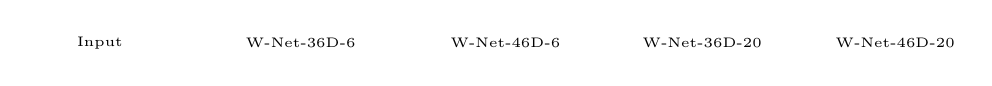
\begin{tikzpicture}
        \node[align=center] at (0, 0) {};
        \node[align=center] at (0.8, 0) {\tiny Input};
        \node[align=center] at (3.35, 0) {\tiny W-Net-36D-6};
        \node[align=center] at (5.95, 0) {\tiny W-Net-46D-6};
        \node[align=center] at (8.45, 0) {\tiny W-Net-36D-20};
        \node[align=center] at (10.9, 0) {\tiny W-Net-46D-20};
    \end{tikzpicture}
    \caption{Selected predictions of different configurations of W-Net}
    \label{fig:wnet_prediction_images}
\end{figure}

It is clearly visible that most configurations did not learn a broad variety of classes. The predictions show mostly one dominant class and sporadic occurances of other classes. Especially for the configurations with 20 available classes this is surprising. They do not make use of the available feature space to encode more information of the original image. This is probably the reason why those configuration also were not able to reconstruct the original images properly.

For the configurations with 6 available classes, the reconstructions look much better. Especially \texttt{W-Net-46D-6} reassembles the rough structure of the original image. This is also the only configuration that makes notable use of at least two of the available classes. But still, four classes remain mostly unused.

In summary, the results of W-Net were very disappointing. Before any of the results could be used to solve the real segmentation challenge, the output would have to be post-processed. This includes merging over-segmented classes and mapping the identified classes to the predefined ones. Due to the poor segmentation results this step was omitted.

\subsection{Discussion}
\label{sec:segmentation_discussion}
The W-Net reference architecture turned out to perform very poorly. With the unsupervised training, the goal was to come up with segmentation classes that were not bound to any human preconceptions. This should also help to gather more insight into the data set in order to uncover potential improvements. However, the W-Net models did not learn any clear differentiation between classes and did not even consume the whole feature space that they were assigned. For those reasons, the W-Net approach was not very effective and is not pursued any further throughout the thesis.

The results of both U-Net and FC-DenseNet were much better in general. The experiments showed that both reference architectures are capable to provide decent predictions. Looking at the plain metrics, there is still some space for improvement in both of them. However, this could also be affected by the inaccuracies in the labels (see section~\ref{sec:dataset_considerations}). The visual results show that the predictions in some cases are even more accurate than the labels.

\begin{figure}
    \newcommand{\DiscussionImageWidth}{0.23\textwidth}
    \centering

    \includegraphics[width=\DiscussionImageWidth]{images/segmentation_discussion/images/1.png} \hfill
    \includegraphics[width=\DiscussionImageWidth]{images/segmentation_discussion/labels/1.png} \hfill
    \includegraphics[width=\DiscussionImageWidth]{images/segmentation_discussion/unet/1.png} \hfill
    \includegraphics[width=\DiscussionImageWidth]{images/segmentation_discussion/densenet/1.png}

    \vspace{2mm}
    \includegraphics[width=\DiscussionImageWidth]{images/segmentation_discussion/images/2.png} \hfill
    \includegraphics[width=\DiscussionImageWidth]{images/segmentation_discussion/labels/2.png} \hfill
    \includegraphics[width=\DiscussionImageWidth]{images/segmentation_discussion/unet/2.png} \hfill
    \includegraphics[width=\DiscussionImageWidth]{images/segmentation_discussion/densenet/2.png}

    \vspace{2mm}
    \includegraphics[width=\DiscussionImageWidth]{images/segmentation_discussion/images/3.png} \hfill
    \includegraphics[width=\DiscussionImageWidth]{images/segmentation_discussion/labels/3.png} \hfill
    \includegraphics[width=\DiscussionImageWidth]{images/segmentation_discussion/unet/3.png} \hfill
    \includegraphics[width=\DiscussionImageWidth]{images/segmentation_discussion/densenet/3.png}

    \begin{tikzpicture}
        \node[align=center] at (0, 0) {};
        \node[align=center] at (0.5, 0) {\tiny Input};
        \node[align=center] at (4.4, 0) {\tiny Label};
        \node[align=center] at (8.3, 0) {\tiny U-Net-23D};
        \node[align=center] at (12, 0) {\tiny FCDN-67D};
    \end{tikzpicture}
    \caption{Large scale predictions of FC-DenseNet-67D and U-Net-23D}
    \label{fig:segmentation_discussion}
\end{figure}

So far, only very small areas have been looked at. In a more practical use case, the predictions would cover huge areas. Hence, figure~\ref{fig:segmentation_discussion} depict the predictions of larger areas, where each of the images covers around $580\times 580$ meters. It shows the original image and label, as well as the visualized predictions of \texttt{U-Net-23D} and \texttt{FCDN-67D}. Those configurations were chosen because they returned the best results in their individual reference architecture (see sections~\ref{sec:unet_experiments} and~\ref{sec:densenet_experiments}).

The similarities between the labels and \texttt{U-Net-23D} predictions are clearly visible. The general outlines of the class segments show only minor differences compared to the labels. This is especially true for the classes \texttt{buildings}, \texttt{forest} and \texttt{agriculture}, which reflects the expected behavior. Since these are the three most dominant classes throughout the data set, lots of good training examples are available.

Also, \texttt{U-Net-23D} provides very accurate predictions for the \texttt{water} class. In contrast to the labels, even small islands in the river are detected correctly. However, there are some false positives for this class when it come to highly saturated green grass, such as on sports fields.

The other two classes, namely \texttt{traffic} and \texttt{urban greens}, are not predicted properly by \texttt{U-Net-23D}. For the both classes this matches the expectations, since they both were labelled rather poorly in the data set. Most roads and traffic areas were not even labelled as \texttt{traffic} class, which makes it almost impossible for the models to learn the correlations correctly. For \texttt{urban greens} the reasoning is similar: Since this class mostly includes parks and sports facilities, it is easily confused with either the \texttt{agriculture} or \texttt{buildings} classes. This is exactly what happens in the model's predictions.

With regards to the classes, the predictions of \texttt{FCDN-67D} can be explained in the same way. However, there is one major difference in the predictions of the two models: \texttt{FCDN-67D} is much more sensitive to fine-grained segments. Especially for the \texttt{buildings} class this can be observed. \texttt{FCDN-67D} distinguishes between single houses and the green spaces between them. In this aspect the predictions are even better than the labels in the data set.

On the other hand, the predictions of \texttt{FCDN-67D} seem very fragmented in some cases, for example between the \texttt{agriculture} and \texttt{forest} classes. The transitions between those two are not really sharp but rather jagged and fissured. To some extent this represents the real situation, because oftentimes there are no clear borders between forest and grassland.

In terms of inference speed \texttt{U-Net-23D} is slightly faster than \texttt{FCDN-67D}. Each image in figure~\ref{fig:segmentation_discussion} took around $9~\text{s}$ to process with \texttt{U-Net-23D}. In contrast, \texttt{FCDN-67D} took around $11~\text{s}$ per image. All measurements were executed on a NVIDIA GeForce GTX 1080 Ti graphics card\footnote{More details on the hardware can be found in appendix~\ref{app:tools_hardware}}.

This is surprising, because \texttt{U-Net-23D} has more than four times the number of parameters compared to \texttt{FCDN-67D} ($16.6~\text{M}$ vs.\ $4.0~\text{M}$). With \texttt{U-Net-23D} however, the parameters are spread across only $23$ convolutional layers, whereas in \texttt{FCDN-67D} there are $67$ layers. Therefore, the calculations in \texttt{U-Net-23D} can better be executed in parallel.

In total, both configuration yield remarkable results for the segmentation challenge. Since the predictions of \texttt{U-Net-23D} are less factured, it might be easier to find suitable emergency landing fields in the huge contiguous areas. However, the predictions might lack precise information of rather small objects. In that regard, the predictions from \texttt{FCDN-67D} are more beneficial.

\subsection{Deployment}
The two models \texttt{U-Net-23D} and \texttt{FCDN-67D} are also provided as Docker Images in~\cite{thesis-code20}. The latest versions of the images can also be found in the public Docker Hub repository \texttt{imageseg/terrain-segmentation}\footnote{\url{https://hub.docker.com/r/imageseg/terrain-segmentation}} The images bundle together all dependencies like the Python interpreter, required Python packages and also the models with the trained weights. This makes it easy to use the models for inference.

The functionality of the images was deliberately kept simple, as they are for demonstration purposes only. The input consists of PNG files with RGB color scheme. The output is also rendered in PNG files, where the class segments are color-encoded as explained in section~\ref{sec:prepare_labels}. All pre- and postprocessing steps are performed automatically inside the Docker container.

For this process, two directories have to be mounted when running a container from the Docker image. The \texttt{/images} directory should contain all input images. All PNG files in this directory will be fed into the model once the container is ready. The predicted results are then written to the \texttt{/predictions} directory. For each input file, a corresponding output file with the same name is created. The container is shut down as soon as all given images are processed.

This workflow is for demonstration purposes only and is not optimized for production use. Starting and stopping Docker containers is a big overhead, because TensorFlow needs some time to ramp up and load the models. For that reason, other options have to be evaluated for production use of the models, like e.~g. TensorFlow Serving\footnote{\url{https://www.tensorflow.org/tfx/guide/serving}} This is a production-ready system for serving TensorFlow models with a standardized interface.

However, the interfaces of TensorFlow Serving only work with tensor objects. Although the interface can be used directly, it makes sense to embed it in a pipeline. That allows to perform pre- and postprocessing steps independently from the model inference. The pipeline can then be connected to other system, e.~g. a PostgreSQL database. This enables the efficient processing of even large volumes of data.

\newpage
